\documentclass[11pt]{article}

\usepackage{url}
\usepackage{color}
\usepackage{float}
\usepackage[format=hang,labelfont=bf,font=small]{caption}
\usepackage{array}
\usepackage{xcolor}
\usepackage{booktabs}
\usepackage[T1]{fontenc}
\usepackage[utf8]{inputenc}
\usepackage[english]{babel}
\usepackage[margin=1in]{geometry}
\usepackage{colortbl}
\usepackage{hyperref}
\usepackage{spreadtab}
\usepackage{longtable}
\usepackage{pdflscape}
\usepackage{subcaption}
\usepackage{amsmath, amsthm, amssymb, amsfonts}
\usepackage{multirow}
\usepackage{graphicx}
\setlength{\parindent}{0cm}

\begin{document}

\title{Deep Learning: Homework 2}
\author{Hugo Mantinhas 95592, João Silveira 95597}

\maketitle

\section*{Work Division}

All group members collaborated on every question in this assignment, leading to an equitable distribution of the workload between each pair.

\section*{Question 1}

\subsection*{1.}

The computational complexity of the self-attention layer of a transformer with a single attention head is \(O(L^2D)\), where \(L\) is the sequence length and \(D\) is the hidden size. In order to break down the complexity of this layer, it is important to note that the complexity of matrix multiplication of two matrices of dimensions \(n \times m\) and \(m \times p\) is \(O(nmp)\). This computation can be broken down into three main operations:

\begin{itemize}
    \item \textbf{Matrix multiplication between \(Q\) and \(K^T\):} This operation has complexity \(O(L^2D)\), since \(Q\) is of size \(L \times D\) and \(K^T\) is of size \(D \times L\).
    \item \textbf{Softmax:} This operation has complexity \(O(L^2)\), since it is applied to a matrix of size \(L \times L\).
    \item \textbf{Matrix multiplication between \(Softmax(QK^T)\) and \(V\):} This operation has complexity \(O(L^2D)\), since the result of the previous operation is of size \(L \times L\) and \(V\) is of size \(L \times D\).
\end{itemize}

Therefore, the overall complexity of the self-attention layer is given by:

\[
    O(L^2D) + O(L^2) + O(L^2D) = O(L^2D)
\]

This can be problematic for long sequences due to the quadratic dependence on the sequence length \(L\). This makes the self-attention layer computationally expensive and increasingly impractical for very long sequences.

\subsection*{2.}

The third expansion for the McLaurin series for approximating the exponential function $e^z$ is expressed as follows:

\begin{equation}
    e^z \approx 1 + z + \frac{z^2}{2}
    \label{q1:2-mclaurin}
\end{equation}

Applying this approximation to \(e^{q^Tk}\), where \(q, k \in \mathbb{R}^D\), yields:

\[
    e^{q^Tk} \approx 1 + q^Tk + \frac{(q^Tk)^2}{2}
\]

Now, notice the that following is true, according to the multinomial theorem~\footnote{\url{https://en.wikipedia.org/wiki/Multinomial_theorem}}:

\[
    (\sum_{i}{a_i})^2 = \sum_{i}{a_i^2} + 2 \sum_{i < j}{a_ia_j}
\]

Applying this theorem, we can expand \((q^T k)^2\) as follows:

\[
    (q^Tk)^2 = \sum_{i=1}^{D}{(q_i k_i)}^2 + 2 \sum_{i < j}^{D}{q_i k_i q_j k_j}
\]

Which, when reorganized to make the feature map derivation more clear, looks as follows:

\[
    (q^Tk)^2 = \sum_{i=1}^{D}{q_i^2 k_i^2} + 2 \sum_{i < j}^{D}{q_i q_j k_i k_j}
\]

Thus, we get the final approximation for \(e^{q^Tk}\):

\[
    e^{q^Tk} \approx 1 + \sum_{i=1}^{D}{q_i k_i} + \frac{\sum_{i=1}^{D}{q_i^2 k_i^2}}{2} + \sum_{i < j}^{D}{q_i q_j k_i k_j}
\]

Finally, to capture this approximation through a feature map \(\phi: \mathbb{R}^D \rightarrow \mathbb{R}^M\), we define:

\[
    \phi(x) =
    \begin{bmatrix}
        1                       \\

        x_1                     \\
        \vdots                  \\
        x_D                     \\

        \frac{1}{\sqrt{2}}x_1^2 \\
        \vdots                  \\
        \frac{1}{\sqrt{2}}x_D^2 \\

        x_1x_2                  \\
        \vdots                  \\
        x_{D-1}x_D
    \end{bmatrix}
\]

Regarding the dimensionality \(M\), we can invoke the multinomial theorem's result for the number of coefficients, in order to calculate the number of coefficients of equation \ref{q1:2-mclaurin}.

\[
    M = 1 + D + \binom{2 + D - 1}{D - 1} = 1 + D + \frac{(D+1)D}{2}
\]

Lastly, for the scenario where $K \geq 3$ terms are employed in the McLaurin series expansion, the dimensionality $M$ can be generalized. Similarly as above, we can also employ the multinomial theorem for this case:

\[
    M = 1 + D + \sum_{J=2}^{K}{\binom{J + D - 1}{D - 1}}
\]

\subsection*{3.}

We have the following statements as true:

\[
    exp(q^Tk) \approx \phi(q)^T \phi(k)
\]

\[
    Z = Softmax(QK^T)V
\]

For conciseness, we will use the following notation:

\[
    S = Softmax(QK^T)
\]

Since, for the self-attention layer, the soft-max operates row-wise, we get:

\[
    S = Softmax(QK^T) \Leftrightarrow S_{ij} = \frac{exp((QK^T)_{ij})}{\sum_l{exp((QK^T)_{il})}} = \frac{exp(q_i^T k_j)}{\sum_l{exp(q_i^T k_l)}}
\]

Now, taking into consideration the initial approximation, we can rewrite it as:

\[
    S_{ij} \approx \frac{\phi(q_i)^T \phi(k_j)}{\sum_l{\phi(q_i)^T \phi(k_l)}}  = \frac{\phi(q_i)^T \phi(k_j)}{(\Phi(K)\phi(q_i))^T 1_L}  = \frac{\phi(q_i)^T \phi(k_j)}{\phi(q_i)^T \Phi(K)^T 1_L}  = \frac{(\Phi(Q) \Phi(K)^T)_{ij}}{\phi(q_i)^T \Phi(K)^T 1_L}
\]

Notice how we can rewrite the bottom part as a diagonal matrix indexation:

\[
    S_{ij} \approx \frac{(\Phi(Q) \Phi(K)^T)_{ij}}{(\Phi(Q) \Phi(K)^T 1_L)_{i}}  = \frac{(\Phi(Q) \Phi(K)^T)_{ij}}{Diag((\Phi(Q) \Phi(K)^T 1_L))_{ii}}  = \frac{(\Phi(Q) \Phi(K)^T)_{ij}}{D_{ii}}
\]

Now, because matrix D is diagonal, inverting this matrix consists in simply inverting each of the elements in the diagonal of D. This means we can generalize by turning $\frac{1}{D_{ii}}$ to $D^{-1}_{ii}$:

\[
    S_{ij} \approx (D^{-1})_{ii} {(\Phi(Q) \Phi(K)^T)_{ij}}
\]

So, finally:

\[
    S \approx D^{-1} \Phi(Q) \Phi(K)^T \Rightarrow Z \approx D^{-1} \Phi(Q) \Phi(K)^T V
\]

\subsection*{4.}

Exploiting the above approximation allows us to simplify the computation and achieve a linear computational complexity in terms of L. Let's break down the major steps for the following computation:

\[
    Z \approx D^{-1} \Phi(Q) \Phi(K)^T V
\]


This computation requires three main steps:

\begin{enumerate}
    \item Computing the diagonal matrix $D$
    \item Computing the inverse $D^{-1}$
    \item Computing the final dot product $D^{-1} \Phi(Q) \Phi(K)^T V$
\end{enumerate}

Starting with the matrix $D$:

\[
    D = Diag(\Phi(Q) \Phi(K)^T 1_L) = Diag(\Phi(Q) X_1)
\]

Starting from the right, the dot product $\Phi(K)^T 1_L$, of matrices sized $M \times L$ and $L \times 1$, respectively, results in a new matrix $X_{1}$, of size $M\times 1$, with a computational complexity of $O(M \times L \times 1) = O(M\times L)$

\[
    Diag(\Phi(Q) X_1) = Diag(X_2)
\]

Starting from the right, the dot product $\Phi(Q) X_1$, of matrices sized $L\times M$ and $M\times 1$, respectively, results in a new matrix $X_{2}$, of size $L \times 1$, with a computational complexity of $O(L\times M \times 1) = O(M\times L)$

\[
    Diag(X_2 ) = D
\]

Computing the $Diag$ function, in practice, doesn't require a matrix of size $L \times L$ matrix to be allocated. Instead, the same vector of size $L \times 1$ can be reused with the exception that all the computations, from now on, behave as if the vector were the diagonal in a diagonal matrix of size $L \times L$. This way, the cost of performing the $Diag$ function could be $O(L)$, or even $O(1)$. Moreover, given that $D$ is a diagonal matrix, inverting it only consists of traversing its diagonal, which has a size of $L$. For this reason, the computational complexity of calculating $D^{-1}$ is also $O(L)$. Lastly, for computing the final dot product:

\[
    Z \approx D^{-1} \Phi(Q) \Phi(K)^T V = D^{-1} \Phi(Q) X_3
\]

Starting from the right, the dot product $\Phi(K)^T V$, of matrices sized $M\times L$ and $L\times D$, respectively, results in a new matrix $X_{3}$, of size $M \times D$, with a computational complexity of $O(M\times L \times D)$.

\[
    D^{-1} \Phi(Q) X_3 = D^{-1} X_4
\]

Starting from the right, the dot product $\Phi(Q) X_3$, of matrices sized $L\times M$ and $M\times D$, respectively, results in a new matrix $X_{4}$, of size $L \times D$, with a computational complexity of $O(L\times M \times D)$.

\[
    D^{-1} X_4 = Z
\]

Finally, we must calculate the dot product of $D^{-1} X_4$, of matrices sized $L\times L$ and $L\times D$, respectively, which results in the final result $Z$. However, unlike the previous matrix multiplications, the left element in this case is a diagonal matrix. Thus, the computational complexity can be trivially reduced to $O(L\times D)$. Analyzing all these complexities, we get that there are two operations with a strictly bigger complexity than the others: the complexity of $O(L\times M\times D)$, which will be the complexity of this operation. In conclusion, the computational complexity depends linearly on $L$, $M$ and $D$.

\section*{Question 2}

\subsection*{1.}

The best configuration has a learning rate of $0.01$. It provided the best results in terms of final test accuracy: $0.8488$.

\begin{figure}[H]
    \hspace{0.025\linewidth}
    \begin{subfigure}{0.45\linewidth}
        \centering
        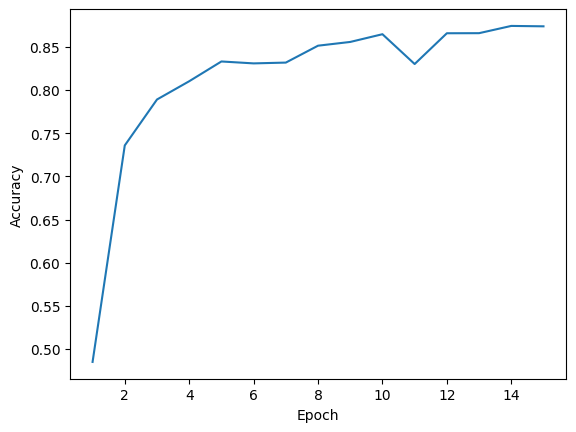
\includegraphics[width=\linewidth]{../data/q2/1/0.01.acc.png}
        \caption{Validation accuracies for learning rate of 0.01 with max pooling}
    \end{subfigure}
    \hspace{0.05\linewidth}
    \begin{subfigure}{0.45\linewidth}
        \centering
        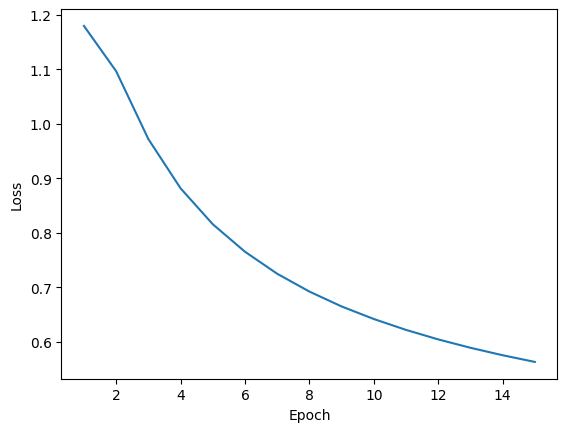
\includegraphics[width=\linewidth]{../data/q2/1/0.01.loss.png}
        \caption{Losses as a function of the number of epochs for learning rate of 0.01 with max pooling}
    \end{subfigure}
\end{figure}

\subsection*{2.}

Using the optimal hyperparameters found in the previous question, that is, with the learning rate of $0.01$, we trained the model for 15 epochs and obtained a final test accuracy of $0.8299$.

\begin{figure}[H]
    \hspace{0.025\linewidth}
    \begin{subfigure}{0.45\linewidth}
        \centering
        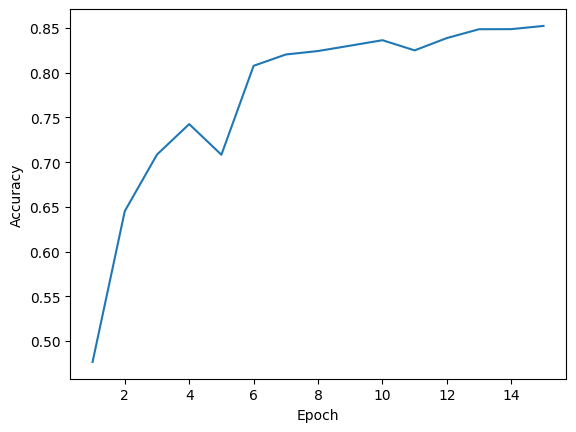
\includegraphics[width=\linewidth]{../data/q2/2/0.01.acc.png}
        \caption{Validation accuracies for learning rate of 0.01 without max pooling}
    \end{subfigure}
    \hspace{0.05\linewidth}
    \begin{subfigure}{0.45\linewidth}
        \centering
        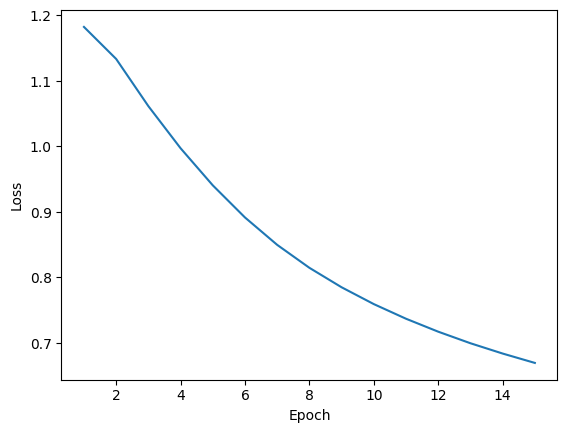
\includegraphics[width=\linewidth]{../data/q2/2/0.01.loss.png}
        \caption{Losses for learning rate of 0.01 without max pooling}
    \end{subfigure}
\end{figure}

\subsection*{3.}

The number of trainable parameters ($225618$) remains unchanged between both CNNs. Consequently, for the training stage, both CNNs have the same expressivity to adjust to data. The more significant difference comes from the application, or absence, of the max pooling layer. The max pooling layer provides many benefits that can justify the model's higher performance. Max pooling will select the highest value of each region and store it, discarding the remaining values. This will discard a lot of potentially less important information and noise, and only keep the highest values, which carry meaning in our network. Max pooling will, inevitably, reduce the spatial dimensions of the input data, however, by definition of the max function, it will always preserve the highest value across pools. This can provide the model translation, rotation, and scale invariance, an important property when classifying images.

\section*{Question 3}

\subsection*{1.}

\begin{figure}[H]
    \hspace{0.025\linewidth}
    \begin{subfigure}{0.45\linewidth}
        \centering
        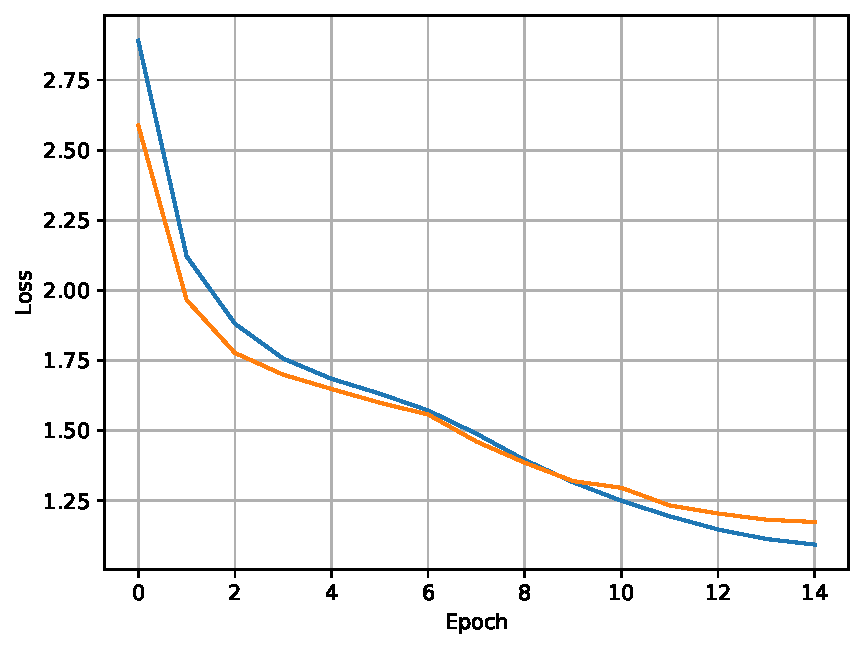
\includegraphics[width=\linewidth]{../data/q3/1/loss__train_val.pdf}
        \caption{Training and validation losses, in blue and orange, respectively}
    \end{subfigure}
    \hspace{0.05\linewidth}
    \begin{subfigure}{0.45\linewidth}
        \centering
        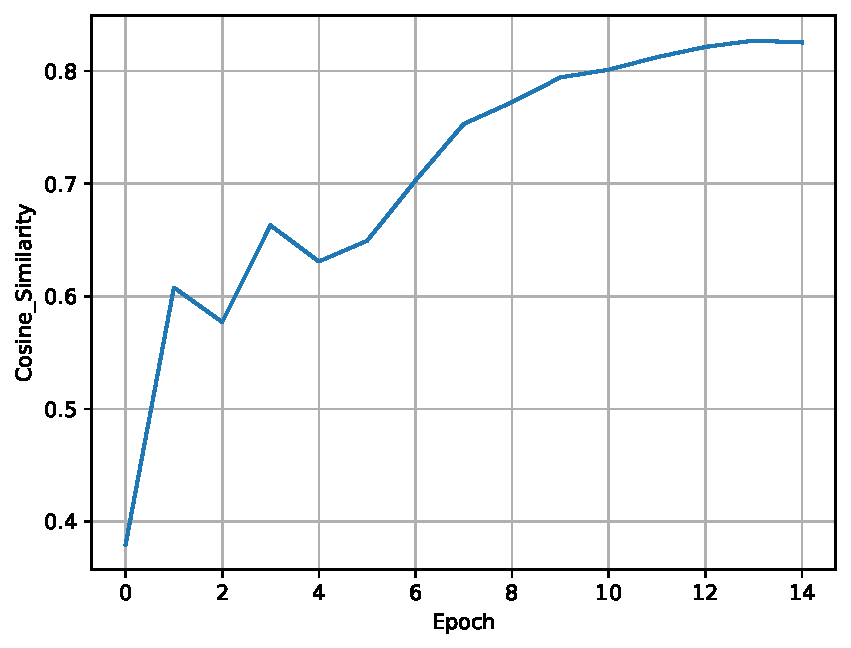
\includegraphics[width=\linewidth]{../data/q3/1/cosine_similarity__val.pdf}
        \caption{Cosine similarity scores for the validation data-set}
    \end{subfigure}

    \vspace{1cm}

    \hspace{0.025\linewidth}
    \begin{subfigure}{0.45\linewidth}
        \centering
        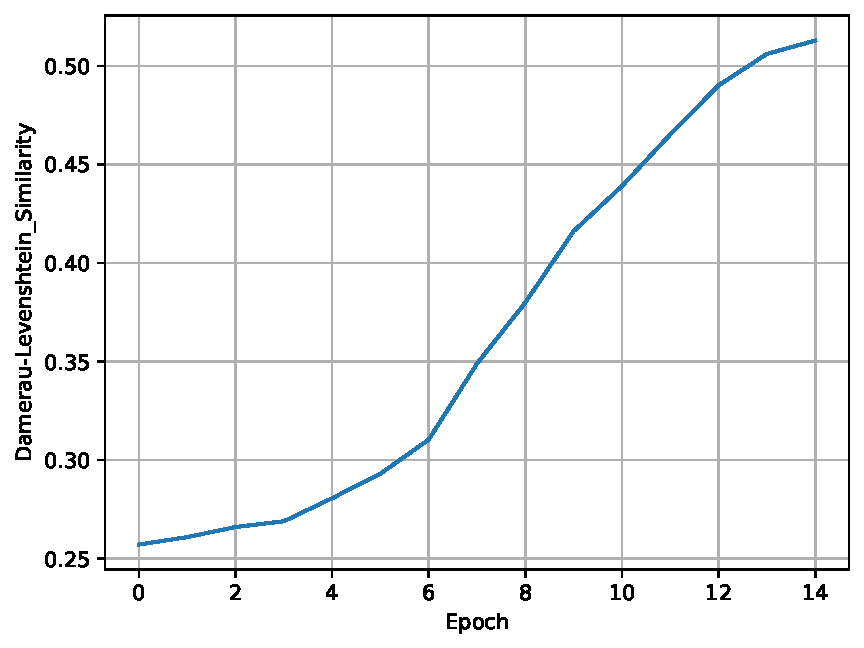
\includegraphics[width=\linewidth]{../data/q3/1/damerau-levenshtein_similarity__val.pdf}
        \caption{Damerau-Levenshtein similarity scores for the validation data-set}
    \end{subfigure}
    \hspace{0.05\linewidth}
    \begin{subfigure}{0.45\linewidth}
        \centering
        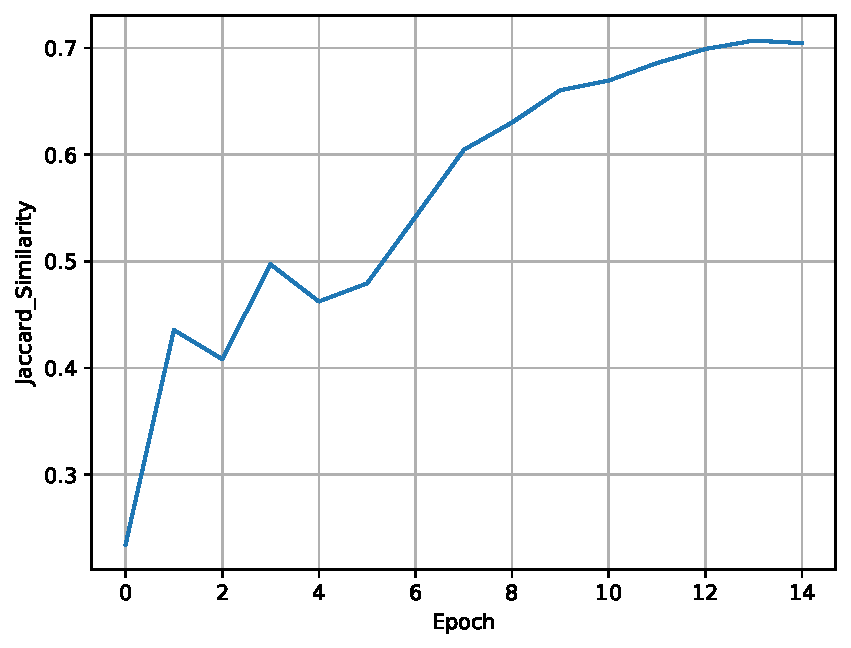
\includegraphics[width=\linewidth]{../data/q3/1/jaccard_similarity__val.pdf}
        \caption{Jaccard similarity scores for the validation data-set}
    \end{subfigure}
\end{figure}

\begin{table}[H]
    \centering
    \begin{tabular}{cc}
        \toprule
        \textbf{Metric}          & \textbf{Test Score} \\
        \midrule
        Loss                     & 1.182828904652014   \\
        Jaccard Sim.             & 0.7149178437842456  \\
        Cosine Sim.              & 0.8324116011552667  \\
        Damerau-Levenshtein Sim. & 0.5087067982887039  \\
        \bottomrule
    \end{tabular}
    \caption{Obtained metrics for the test data-set, using \texttt{TextDecoderRecurrent}}
\end{table}

\subsection*{2.}

\begin{figure}[H]
    \hspace{0.025\linewidth}
    \begin{subfigure}{0.45\linewidth}
        \centering
        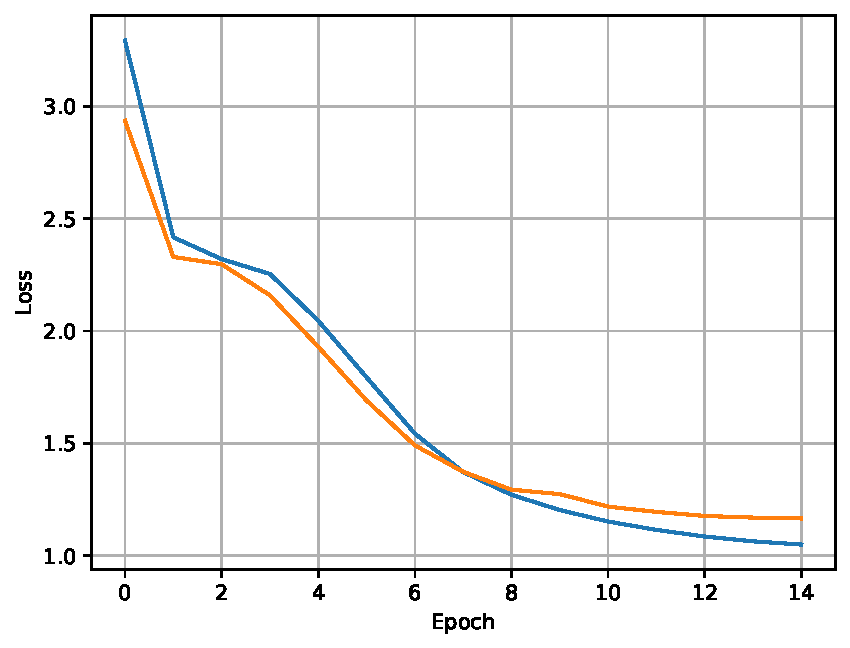
\includegraphics[width=\linewidth]{../data/q3/2/loss__train_val.pdf}
        \caption{Training and validation losses, in blue and orange, respectively}
    \end{subfigure}
    \hspace{0.05\linewidth}
    \begin{subfigure}{0.45\linewidth}
        \centering
        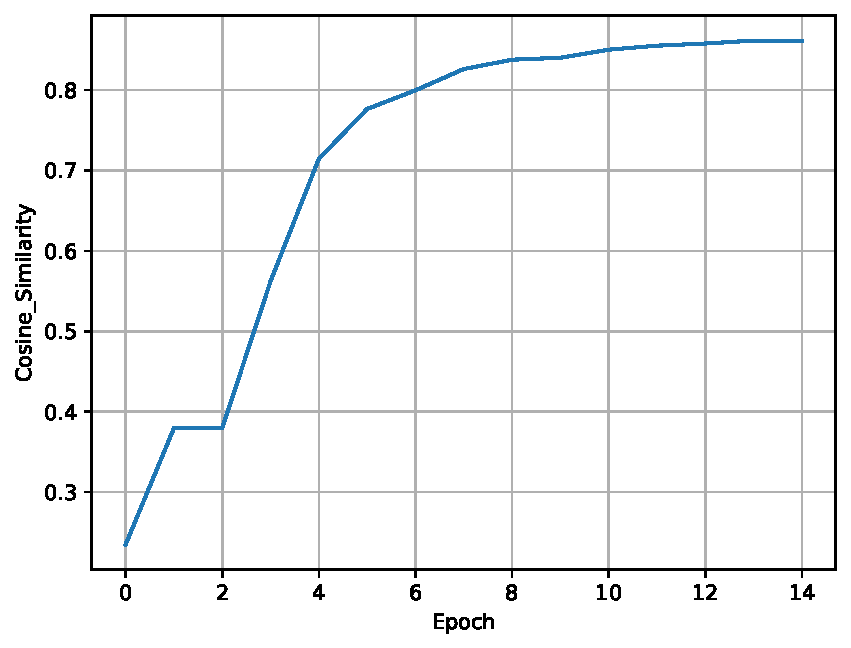
\includegraphics[width=\linewidth]{../data/q3/2/cosine_similarity__val.pdf}
        \caption{Cosine similarity scores for the validation data-set}
    \end{subfigure}

    \vspace{1cm}

    \hspace{0.025\linewidth}
    \begin{subfigure}{0.45\linewidth}
        \centering
        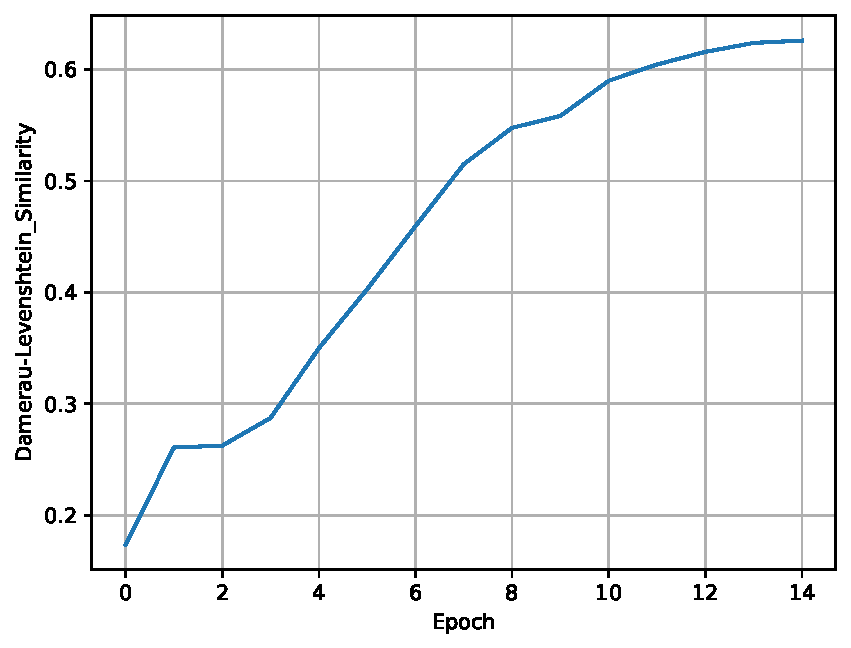
\includegraphics[width=\linewidth]{../data/q3/2/damerau-levenshtein_similarity__val.pdf}
        \caption{Damerau-Levenshtein similarity scores for the validation data-set}
    \end{subfigure}
    \hspace{0.05\linewidth}
    \begin{subfigure}{0.45\linewidth}
        \centering
        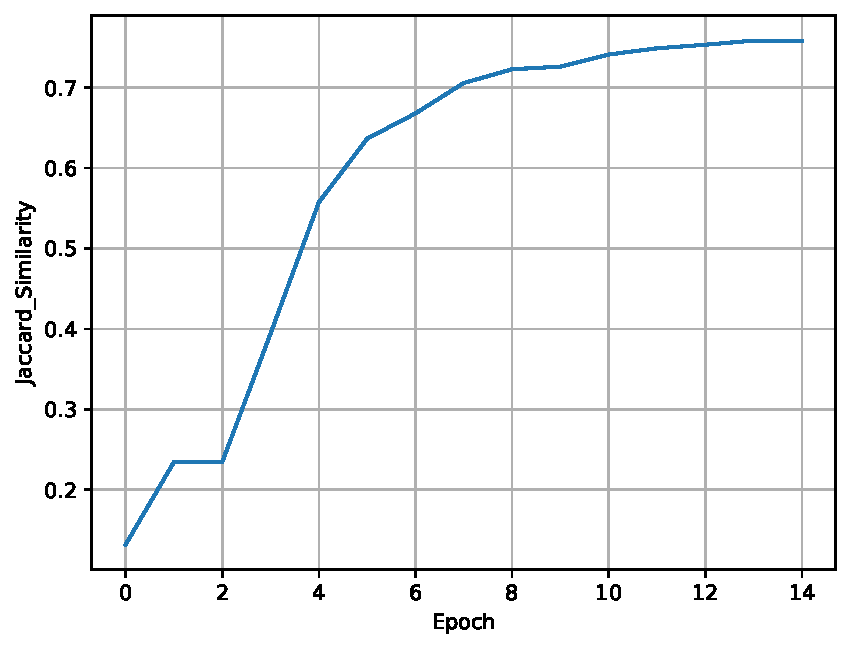
\includegraphics[width=\linewidth]{../data/q3/2/jaccard_similarity__val.pdf}
        \caption{Jaccard similarity scores for the validation data-set}
    \end{subfigure}
\end{figure}

\begin{table}[H]
    \centering
    \begin{tabular}{cc}
        \toprule
        \textbf{Metric}          & \textbf{Test Score} \\
        \midrule
        Loss                     & 1.1605787364447988  \\
        Jaccard Sim.             & 0.7654325449316394  \\
        Cosine Sim.              & 0.8658540860411359  \\
        Damerau-Levenshtein Sim. & 0.6346722294393772  \\
        \bottomrule
    \end{tabular}
    \caption{Obtained metrics for the test data-set, using \texttt{TextDecoderTransformer}}
\end{table}

\subsection*{3.}

The LSTM is a type of recurrent neural network (RNN) that is designed to address the vanishing gradient problem, allowing it to better capture long-range dependencies in sequential data. The LSTM processes input sequences sequentially, one element at a time. For storing information over time, LSTMs use memory cells with three gates that control the flow of information: the input gate, the forget gate, and the output gate. The input gate determines which parts of the input should be stored in the memory cell. The forget gate controls which information in the memory cell should be discarded. Lastly, the output gate controls what information from the memory cell should be output to the next step in the sequence.

The attention mechanism, on the other hand, processes the entire input sequence in parallel. In this model, each element in the sequence can attend to all other elements, enabling the model to capture long-range dependencies more efficiently. In its essence, attention consists of computing attention scores, which indicate the importance of each element in the sequence concerning the current element being processed. Each resulting token is the weighted sum of information from all other elements, including the one being processed. Moreover, transformers often employ multiple attention heads, each capturing different aspects of the relationships in the input sequence.

In summary, while LSTMs process input sequences sequentially with a focus on capturing dependencies using memory cells, attention-based mechanisms process input sequences in parallel, allowing a more efficient capture of long-range dependencies and contextual information. Across all the obtained metrics, the transformer model outperformed the LSTM model. This suggests that the attention mechanism in the transformer is more effective at capturing the relationships between words and their context, which is particularly important for the task of speech recognition.

\subsection*{4.}

For all these similarities, the higher the value, the higher the similarity between the recognized and reference transcriptions. However, they measure similarity very differently. Cosine similarity attempts to compare the vectors that represent the both sentences in a multidimensional space by analyzing the angle between them. Since the closer these two vectors are, the closer their meaning is, cosine similarity is quite good at capturing the semantic similarity between the reference transcriptions and the ones derived from the speech signals. Jaccard similarity, on the other hand, measures the overlap of recognized phonemes between the predicted and reference transcriptions. This is done by calculating the ratio between the correct terms and the total number of terms. A Jaccard similarity of 1 implies a complete overlap of terms, and 0 implies no overlap at all. Lastly, the Damerau-Levenshtein similarity, is a string similarity metric that considers insertions, deletions, substitutions, and transpositions of characters. This similarity metric is used to assess the similarity between the recognized and reference transcriptions at the character level. In summary, all of these metrics are relevant to assess how well the models are performing. In general, the cosine similarity is a good measure of semantic similarity, while the Jaccard and Damerau-Levenshtein similarities are good proxies of phonetic similarity.

\end{document}